\begin{flushright} {\tiny {\color{gray} (tikz\_dssy3D.tex)}} \end{flushright}
%~~~~~~~~~~~~~~~~~~~~~~~~~~~~~~~~~~~~~~~~~~~~~~~~~~~~~~~~~~~~~~~~~~~~~~~~~~~~~~~~~~~~~~~~~~~~~~~~~~

\begin{center}
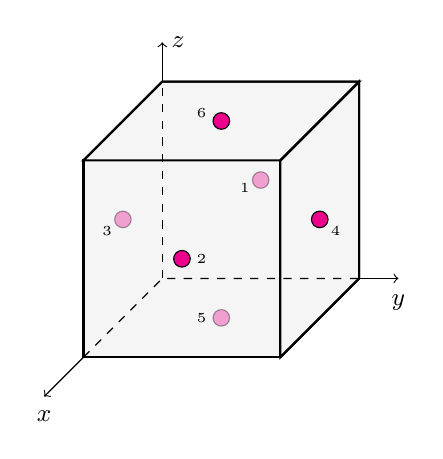
\begin{tikzpicture}

%\draw[step=1cm,gray,very thin] (0,0) grid (8,8); %background grid

\draw[thick,fill=gray!8] (5,1) -- (7.5,1) -- (7.5,3.5) -- (5,3.5) -- cycle;
\draw[thick,fill=gray!8] (7.5,1) -- (8.5,2) -- (8.5,4.5) -- (7.5,3.5) -- cycle;
\draw[thick,fill=gray!8] (5,3.5) -- (7.5,3.5) -- (8.5,4.5) -- (6,4.5) -- cycle;
\draw[thick] (5,3.5) -- (6,4.5) -- (8.5,4.5) -- (8.5,2) -- (7.5,1);
\draw[thick] (7.5,3.5) -- (8.5,4.5) ;
\draw[dashed] (5,1) -- (6,2) -- (8.5,2) ;\draw[dashed] (6,2) -- (6,4.5);


\draw[black,fill=magenta,opacity=0.35] (5.5,2.75)   circle (3pt);
\draw[black,fill=magenta] (8,2.75)   circle (3pt);
\draw[black,fill=magenta,opacity=0.35] (6.75,1.5)   circle (3pt);
\draw[black,fill=magenta] (6.75,4)   circle (3pt);
\draw[black,fill=magenta] (6.25,2.25)   circle (3pt);
\draw[black,fill=magenta,opacity=0.35] (7.25,3.25)   circle (3pt);

\node[] at (7.05,3.15) {\tiny 1};
\node[] at (6.5,2.25) {\tiny 2};
\node[] at (5.3,2.6) {\tiny 3};
\node[] at (8.2,2.6) {\tiny 4};
\node[] at (6.5,1.5) {\tiny 5};
\node[] at (6.5,4.1) {\tiny 6};

\draw[->] (5,1)--(4.5,0.5);
\draw[->] (8.5,2)--(9,2);
\draw[->] (6,4.5)--(6,5);

\node[] at (4.5,0.25) {\small $x$};
\node[] at (9,1.7) {\small $y$};
\node[] at (6.2,5) {\small $z$};

\end{tikzpicture}
\end{center}
